%=================== LaTeX 习题模板(仅含学院与考试信息) ===================
\documentclass[12pt,a4paper]{article}

%----------------- 页面与中文支持 -----------------
\usepackage[margin=2cm]{geometry}    % 设置页边距
\usepackage{ctex}                    % 支持中文
\usepackage{amsmath,amssymb}         % 数学公式与符号
\usepackage{enumitem}                % 自定义列表格式
\usepackage{tikz}
\usetikzlibrary{decorations.pathmorphing}
\usepackage{float} % 支持 [H] 浮动体选项
\usepackage[most]{tcolorbox} % 支持彩色盒子
\usepackage{multirow} % 支持表格多行单元格

%----------------- 页眉页脚 -----------------
\usepackage{fancyhdr}
\pagestyle{fancy}
\fancyhf{}
% 左侧:学院(留空由学生填写)
\lhead{学院:\underline{\hspace{2cm}CCEA\hspace{2cm}}}
% 右侧:考试信息(如“期末考试”、“月考试卷”等,由学生填写)
\rhead{考试:\underline{\hspace{2cm}Fluid Mechanics\hspace{2cm}}}
\cfoot{\thepage}

%----------------- 题目环境 -----------------
\newcounter{question}
\newenvironment{questions}{
    \setcounter{question}{0}
    \section*{Question}
    \begin{enumerate}[leftmargin=1.5em,label={\arabic*.}]
}{
    \end{enumerate}
}

%----------------- 答案环境 -----------------
\newenvironment{answers}{
    \setcounter{question}{0}
    \section*{习题答案}
    \begin{enumerate}[leftmargin=1.5em,label={\arabic*.}]
}{
    \end{enumerate}
}

% 用于每题答案的加粗提示
\newcommand{\answer}[1]{\par\noindent\textbf{Answer:} #1\par\vspace{1em}}

% 定义浅色框样式
\newtcolorbox{mybox}{
    colback=lightgray!20,    % 浅灰色背景(20%透明度)
    colframe=lightgray!50,   % 边框颜色
    boxrule=1pt,             % 边框粗细
    arc=4pt,                 % 圆角弧度
    boxsep=5pt,              % 内边距
    left=6pt, right=6pt,     % 左右边距
    top=6pt, bottom=6pt      % 上下边距
}

%=========================================================

\begin{document}
\section{考试注意事项}

\begin{mybox}
\begin{itemize}
  \item 选择题:None of them,指1个都不对,共28分
  \item 名词解释题:5分 $\times$ 3,共 15分
  \item EGL: \quad 两个画图题 4 + 6 共10分 \\
  HGL:
  \item 47分计算题:包括连续性方程 \quad 伯努力方程 \quad 动量方程 \quad 静压计算
\end{itemize}

总分:100分
\end{mybox}



考试采取全英文作答,中文答案不计分,考试可以带计算器和英汉词典,但是语法错误无关紧要。以下题目和概念来源郑飞飞最后一节课划重点内容,可以参考复习,为了适应英文作答,从现在开始改为英文内容。

本文档将选择题和名词解释题的内容放在一个section下,计算题放在另一个section,同时计算题会覆盖课后习题以及ppt内容。

水银的密度是 $13.6 \times 10^3 \mathrm{kg/m^3}$,水的密度是 $1.0 \times 10^3 \mathrm{kg/m^3}$,水银的比重是 $13.6$。
\[
\gamma_{Hg} = 133.4 \times 10^3 \mathrm{N/m^3} \quad \gamma_{water} = 9.8 \times 10^3 \mathrm{N/m^3}
\]
\newpage

%=================== 题目部分 ===================

\section{Multiple-choice questions\&Term Definition Questions}

\begin{questions}
  \item Describe the differences between fluids and gases.
  \answer{
    Fluids:
    \begin{itemize}
      \item relative smaller distance between molecules(分子)
      \item it's hard to compress
      \item relative fixed volume
      \item the force between molecules is larger than the force between molecules in gases
    \end{itemize}

    Gases:
    \begin{itemize}
      \item relative larger distance between molecules
      \item it's easy to compress
      \item the force between molecules is smaller than the force between molecules in fluids
    \end{itemize}
  }

  \item Describe the Continuum assumption(连续性假设)
  
  \answer{
    The Continuum assumption is the assumption that fluids are continuous media, meaning that they can be treated as continuous distributions of matter without considering the discrete nature of molecules. This allows for the application of classical mechanics to analyze fluid behavior, treating properties like density and velocity as continuous functions rather than discrete values.
  }

  \item Describe Newton's Law of Viscosity(牛顿内摩擦定律),How to distinguish between Newtonian and non-Newtonian fluids?(如何区分牛顿流体和非牛顿流体)
  
  \answer{
    Newton's Law of Viscosity states that the shear stress(剪切应力) between adjacent layers of a fluid is proportional to the velocity gradient(速度梯度) between those layers. Mathematically, it can be expressed as:
    \[
    \tau = \mu \frac{du}{dy}
    \]
    where $\tau$ is the shear stress, $\mu$ is the dynamic viscosity, $du$ is the change in velocity, and $dy$ is the change in distance between the layers.

    Newtonian fluids are those that obey this law, meaning their viscosity remains constant regardless of the shear rate. Examples include water and air. Non-Newtonian fluids, on the other hand, do not follow this law; their viscosity can change with the shear rate. Examples include ketchup and blood.
  }

  \item Describe the Mass force and Surface force(表面力)
  
  \answer{
    Mass Force (质量力) is the force distributed throughout the control body. Its magnitude(大小) is proportional(成比例的) to the mass of the control body, and for homogeneous fluid it is also directly proportional to fluid volume, also known as body force. Unit: N.
  
    Surface Force (表面力) is the force distributed on the surface of the control body. It incudes the presure force and the shear stress.  The unit of surface force is also N.
    }

    \item Describe the Capillary action
    
    \answer{
      Capillary action(毛细现象) in small tubes which involve a liquid-gas-solid interface is caused by surface tension. The fluid is either drawn up the tube or pushed down.
    }

    \item When can a surface be called an equipressure surface?
    
    \answer{
      1. At rest \quad 2. Connection \quad 3. the same homogenous(同一介质) fluid \quad 4. The only mass force is gravity \quad 5. At the same level .
    }

    \item Introduce the concept of  Elevation Head 、 Piezometric(测压) Height  and Piezometric Head 

    \answer{
      Elevation Head (高程头) is the height of a point above a reference level, typically the datum level. It is denoted as $z$ and is measured in meters.

      Piezometric Height (测压高度) is the height to which a fluid will rise in a piezometer tube due to pressure. It is the sum of the elevation head and the pressure head, given by:
      \[
      Piezometric \ Height = \frac{p}{\gamma}
      \]
      Piezometric Head (测压头) is represents total potential energy 
per unit weight of fluid,given by:
      \[
      Piezometric \ Head = z + \frac{p}{\gamma}
      \]
      where $z$ is the elevation head, $p$ is the pressure, and $\gamma$ is the specific weight of the fluid. It is also measured in meters.
    }

  \item Introduce Bernoulli's Equation
  
  \answer{
    Bernoulli's Equation is a fundamental principle in fluid mechanics that describes the conservation of energy in a flowing fluid. It states that the total mechanical energy along a streamline is constant, and can be expressed as:
    \[
    P + \frac{1}{2} \rho v^2 + \rho g z = \text{constant}
    \]
    where $P$ is the pressure, $\rho$ is the fluid density, $v$ is the flow velocity, $g$ is the acceleration due to gravity, and $z$ is the elevation head. This equation applies to incompressible, non-viscous fluids in steady flow.
  }

    \item Introduce the concept of Geometric Center(形心) and the center of Pressure(压心)

    \answer{
      The Geometric Center (形心) of a surface is the point where the geometric center of the area lies. It is the average position of all points in the area and is calculated as the centroid of the shape.

      The Center of Pressure (压心) is the point on a submerged surface where the total pressure force acts. It is not necessarily at the geometric center, especially for non-uniform pressure distributions. The center of pressure is always located below the geometric center for submerged surfaces due to the hydrostatic pressure distribution.

      For an inclined geometric body,we can calculate the depth of the Geometric Center as:
      \[
      F= \gamma h_c A
      \]
      where $F$ is the total force acting on the surface, $\gamma$ is the specific weight of the fluid, $h_c$ is the depth of the geometric center, and $A$ is the area of the surface.
      and we also know that:
      \[
      dF = \gamma h dA= \gamma y \sin \theta dA,Therefore \ F = \int_A \gamma y \sin \theta dA
      \]
      For the center of pressure, we can calculate the depth as:
      \[
      F y_p = \int_A y \gamma y \sin \theta dA
      \]
      We should remark that the y coordinate of the center of pressure is always below the y coordinate of the geometric center, and the distance between them is given by:
      \[
      h_p = \frac{I_G}{A h_c} + h_c
      \]
      where $I_G$ is the second moment of area about the horizontal axis through the geometric center, $A$ is the area of the surface, and $h_c$ is the depth of the geometric center.
    
      Also by the knowledge of the center of pressure, If the pressure increases uniformly with depth (hydrostatic pressure distribution), the center of pressure is located at two-thirds of the depth from the free surface.
      }
      \item Introduce the concept of EGL and HGL
  \answer{
  EGL(Energy Grade Line)、TGL(Total Energy Line):$z+\frac{p}{\gamma}+\frac{v^2}{2g}$

HGL(Hydraulic Grade Line, HGL):$z+\frac{p}{\gamma}$
  }

  For example:

  \begin{figure}[H]
    \centering
    \includegraphics[width=0.6\textwidth]{./figures/5.png}
  \end{figure}

  \begin{figure}[H]
    \centering
    \includegraphics[width=0.6\textwidth]{./figures/6.png}
  \end{figure}

  \begin{figure}[H]
    \centering
    \includegraphics[width=0.6\textwidth]{./figures/7.png}
  \end{figure}

  We must note that the turbine is a device that converts the energy of flowing water into mechanical energy, and the pump is a device that converts mechanical energy into the energy of flowing water. The EGL and HGL are used to analyze the energy changes in these devices.
  \begin{figure}[H]
    \centering
    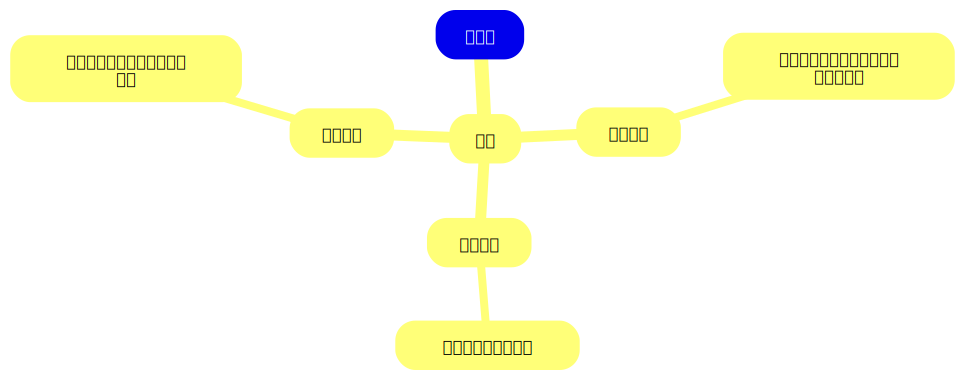
\includegraphics[width=0.6\textwidth]{./figures/13.png}
  \end{figure}

  \begin{figure}[H]
    \centering
    \includegraphics[width=0.6\textwidth]{./figures/14.png}
  \end{figure}

  \begin{figure}[H]
    \centering
    \includegraphics[width=0.6\textwidth]{./figures/15.png}
  \end{figure}

  \begin{figure}[H]
    \centering
    \includegraphics[width=0.6\textwidth]{./figures/16.png}
  \end{figure}

  \begin{figure}[H]
    \centering
    \includegraphics[width=0.6\textwidth]{./figures/17.png}
  \end{figure}

  \begin{figure}[H]
    \centering
    \includegraphics[width=0.6\textwidth]{./figures/18.png}
  \end{figure}
  \item Introduce the basic concepts of the flow
  
  \answer{
  \begin{itemize}
    \item \textbf{Laminar Flow} \\
    Smooth, layered motion with no cross-mixing (low Reynolds number, $Re < 2100$ for pipes).

    \item \textbf{Turbulent Flow} \\
    Chaotic motion with eddies and mixing (high Reynolds number, $Re > 4000$ for pipes).

    \item \textbf{Steady Flow} \\
    Flow parameters (velocity, pressure) remain constant with time ($\frac{\partial}{\partial t} = 0$).

    \item \textbf{Unsteady Flow} \\
    Flow parameters vary with time ($\frac{\partial}{\partial t} \neq 0$), e.g., tidal flows.

    \item \textbf{Uniform Flow} \\
    Velocity remains constant along the flow direction ($\frac{\partial}{\partial s} = 0$).

    \item \textbf{Non-uniform Flow} \\
    Velocity changes along the flow path ($\frac{\partial}{\partial s} \neq 0$), e.g., converging pipes.
\end{itemize}
  }

    \item Introduce Eulerian vs. Lagrangian Descriptions of Fluid Motion
  
    \answer{

      For Eulerian description, we focus on specific points in space and observe how fluid properties change over time at those points. This approach is commonly used in fluid dynamics, where we analyze flow fields and velocity distributions.
      For Lagrangian description, we track individual fluid particles as they move through space and time. This approach is useful for understanding the trajectory of specific particles and their interactions with the surrounding fluid.  
      \[ a_x = \frac{d u_x}{d t} = \frac{\partial u_x}{\partial t} + u_x \frac{\partial u_x}{\partial x} + u_y \frac{\partial u_x}{\partial y} + u_z \frac{\partial u_x}{\partial z} \]
    Derivation steps are as follows:
      \[
\mathbf{a} = \frac{d \mathbf{V}}{d t} = \frac{d \mathbf{V}(x,y,z,t)}{d t} = \frac{\partial \mathbf{V}}{\partial x} \frac{d x}{d t} + \frac{\partial \mathbf{V}}{\partial y} \frac{d y}{d t} + \frac{\partial \mathbf{V}}{\partial z} \frac{d z}{d t} + \frac{\partial \mathbf{V}}{\partial t}
\]
\[
= \frac{\partial \mathbf{V}}{\partial t} + (\mathbf{V} \cdot \nabla) \mathbf{V}
\]
\[
= \left( \frac{\partial u_x}{\partial t}, \frac{\partial u_y}{\partial t}, \frac{\partial u_z}{\partial t} \right) + \left( u_x \frac{\partial}{\partial x} + u_y \frac{\partial}{\partial y} + u_z \frac{\partial}{\partial z} \right) (u_x, u_y, u_z)
\]
For example,
\[
a_x = \frac{\partial u_x}{\partial t} + u_x \frac{\partial u_x}{\partial x} + u_y \frac{\partial u_x}{\partial y} + u_z \frac{\partial u_x}{\partial z}
\]
      }

    \item How to Describe incompressible and compressible flow?
    
    \answer{
      Incompressible flow is characterized by a constant fluid density, meaning that the density does not change with pressure or temperature variations. This is typically applicable to liquids and low-speed gas flows. The continuity equation for incompressible flow can be expressed as:
      \[
      \nabla \cdot \mathbf{V} = 0
      \]
      where $\mathbf{V}$ is the velocity vector.

      Compressible flow, on the other hand, involves significant changes in fluid density due to pressure and temperature variations. This is common in high-speed gas flows, such as those encountered in aerodynamics. The continuity equation for compressible flow can be expressed as:
      \[
      \frac{\partial \rho}{\partial t} + \nabla \cdot (\rho \mathbf{V}) = 0
      \]
      where $\rho$ is the fluid density.

      Also,we can compare the continuity formula of incompressible flow with compressible flow:
      \[
      \nabla \cdot \mathbf{V} = 0 \quad \text{(incompressible flow)}
      \]
      \[
      \frac{\partial \rho}{\partial t} + \nabla \cdot (\rho \mathbf{V}) = 0 \quad \text{(compressible flow)}
      \]

      The deprivation of the continuity equation for compressible flow is as follows:
      
      the rate of mass outflow from a control volume is equal to the rate of mass inflow plus the rate of change of mass within the control volume. This can be expressed mathematically as:
      $$\text{outflow rate} = \nabla \cdot (\rho \mathbf{V})$$
      the mass derivative is given by:
      $$\text{mass derivative} = \frac{\partial \rho}{\partial t} \mathbf{V}$$
      Therefore, the continuity equation for compressible flow can be expressed as:
      \[\frac{\partial \rho}{\partial t} + \nabla \cdot (\rho \mathbf{V}) = 0
      \]
      }

      \item Introduce the concept of Reynolds Number and its significance in fluid mechanics.
      \answer{
        The Reynolds Number (Re) is a dimensionless quantity used to predict flow patterns in fluid mechanics. It is defined as the ratio of inertial forces to viscous forces and is given by:
        \[
        Re = \frac{\rho V L}{\mu}
        \]
        where $\rho$ is the fluid density, $V$ is the characteristic velocity, $L$ is the characteristic length, and $\mu$ is the dynamic viscosity.

        The significance of Reynolds Number lies in its ability to distinguish between laminar and turbulent flow regimes:
        \begin{itemize}
          \item Laminar Flow: Occurs when $Re < 2100$, characterized by smooth, orderly motion with layers of fluid sliding past each other.
          \item Transitional Flow: Occurs when $2100 < Re < 4000$, where flow may switch between laminar and turbulent.
          \item Turbulent Flow: Occurs when $Re > 4000$, characterized by chaotic, irregular motion with eddies and vortices.
        \end{itemize}
        Understanding Reynolds Number helps engineers design systems that can handle different flow conditions effectively.
      }

      \item Introduce the concept of the stream function and the potential function.
      \answer{
        The stream function is a mathematical function used to describe the flow of an incompressible fluid. It is defined such that the velocity components can be derived from it:
        \[
        u = \frac{\partial \psi}{\partial y}, \quad v = -\frac{\partial \psi}{\partial x}
        \]
        where $\psi$ is the stream function, $u$ is the velocity in the x-direction, and $v$ is the velocity in the y-direction. The stream function is constant along streamlines, making it useful for visualizing flow patterns.

        The potential function, on the other hand, is used to describe irrotational flow. It is defined such that the velocity components can be expressed as:
        \[
        u = \frac{\partial \phi}{\partial x}, \quad v = \frac{\partial \phi}{\partial y}
        \]
        where $\phi$ is the potential function. The potential function is constant along equipotential lines, which are perpendicular to streamlines in irrotational flow.
      
          The most important thing is that we can obtain the two function by calculating the velocity field:
        \[
        \psi = \int - v dx +  u dy
        \]
        Also:
        \[
        \phi = \int u dx + v dy
        \]

        Note that the stream function is incompressible flow, while the potential function is irrotational flow. The stream function is used for incompressible flow, while the potential function is used for irrotational flow.

        Now we give some examples of the stream function and the potential function:

        There are velocity fields for two flows as follows:
      }
(a) \( u_x = 1, u_y = 2 \);

(b) \( u_x = 4x, u_y = -4y \).

(1) Is there stream function in flow (a)? If yes, what is the stream function \( \psi \)?

(2) Is there potential function in flow (b)? If yes, what is the potential function \( \phi \)?

  \answer{
    For flow (a), the velocity components are constant:
    \[
    u_x = 1, \quad u_y = 2
    \]
    Since the velocity components are constant, the flow is incompressible. Therefore, we can find the stream function \( \psi \) as follows:
    \[
    \psi = \int - u_y dx + u_x dy = \int -2 dx + 1 dy = -2x + y + C
    \]
    where \( C \) is a constant of integration. Thus, the stream function for flow (a) is:
    \[
    \psi = -2x + y + C
    \]
    For flow (b), the velocity components are:
    \[
    u_x = 4x, \quad u_y = -4y
    \]
    To check if there is a potential function \( \phi \), we need to verify if the flow is irrotational. The flow is irrotational if the curl of the velocity field is zero:
    \[
    \nabla \times \mathbf{V} = \left( \frac{\partial u_y}{\partial x} - \frac{\partial u_x}{\partial y} \right) = 0
    \]
    Calculating the derivatives:
    \[
    \frac{\partial u_y}{\partial x} = 0, \quad \frac{\partial u_x}{\partial y} = 0
    \]
    Since both derivatives are zero, the flow is irrotational. Therefore, we can find the potential function \( \phi \) as follows:
    \[
    \phi = \int u dx + v dy = \int 4x dx + (-4y) dy = 2x^2 - 4y^2 + C
    \]
    where \( C \) is a constant of integration. Thus, the potential function for flow (b) is:
    \[
    \phi = 2x^2 - 4y^2 + C
    \]
  }

    \item Introduction to streamlines and pathlines
    
    \answer{
      Streamlines are lines that are tangent to the velocity vector of the flow at every point, representing the path that a fluid element follows. In steady flow, streamlines do not change over time. They can be visualized by releasing dye into the flow and observing the pattern it forms.

      Pathlines, on the other hand, are the actual paths that individual fluid particles follow over time. In steady flow, streamlines and pathlines coincide, but in unsteady flow, they can differ significantly.
    }

    \item Introduce the type of downhill slope
    
    \answer{
\begin{itemize}
  \item \textbf{Critical Slope} \((S_0 = S_{0c})\)(临界坡):
    \begin{itemize}
      \item When the bed slope of the channel is equal to the critical slope corresponding to a certain discharge.
      \item In a long channel, unstable critical flow will occur.
    \end{itemize}
  \item \textbf{Mild Slope} \((S_0 < S_{0c})\)(缓坡):
    \begin{itemize}
      \item When the bed slope of the channel is less than the critical slope corresponding to a certain discharge.
      \item In a long channel, subcritical flow will occur.
    \end{itemize}
  \item \textbf{Steep Slope} \((S_0 > S_{0c})\)(陡坡):
    \begin{itemize}
      \item When the bed slope of the channel is greater than the critical slope corresponding to a certain discharge.
      \item In a long channel, supercritical flow will occur.
    \end{itemize}
\end{itemize}

    }

    \item Describe the characteristics of rapid flow, tranquil flow, and critical flow(描述急流、缓流和临界流的特征)


\begin{table}[H]
\centering
\renewcommand{\arraystretch}{1.2} % 缩小行高
\setlength{\tabcolsep}{0.5pt} % 缩小列间距
\begin{tabular}{|c|c|c|c|c|}
\hline
\multicolumn{2}{|c|}{\textbf{Classification Index}} & \textbf{Tranquil Flow} & \textbf{Critical Flow} & \textbf{Rapid Flow} \\ \hline
\multirow{5}{*}{\begin{tabular}[c]{@{}c@{}}Uniform or \\ Non-uniform \\ Flow\end{tabular}} 
& Water Depth \(y\) & \(y > y_c\) & \(y = y_c\) & \(y < y_c\) \\ \cline{2-5} 
& Froude Number \(Fr\) & \(Fr < 1.0\) & \(Fr = 1.0\) & \(Fr > 1.0\) \\ \cline{2-5} 
& Position on \(E_s - y\) curve & Upper branch & \(E_s = E_{s_{\min}}\) & Lower branch \\ \cline{2-5} 
& Rate of change of \(E_s\) & Decreases with \(y\) & Minimum & Increases with \(y\) \\ \cline{2-5} 
& Ratio of potential to kinetic energy & Potential $>$ Kinetic & Equal & Kinetic $>$ Potential \\ \hline
\multirow{2}{*}{Uniform Flow} 
& Channel Slope \(S_0\) & \(S_0 < S_{0c}\) & \(S_0 = S_{0c}\) & \(S_0 > S_{0c}\) \\ \cline{2-5} 
& Normal Depth \(y_0\) & \(y_0 > y_c\) & \(y_0 = y_c\) & \(y_0 < y_c\) \\ \hline
\end{tabular}
\caption{Classification of open channel flow: tranquil, critical, and rapid flow}
\end{table}

\begin{figure}[H]
  \centering
  \includegraphics[width=0.4\textwidth]{./figures/29.png}
  \caption{Classification of open channel flow: tranquil, critical, and rapid flow}
\end{figure}

\item Introduce the concept of Weir Flow

\answer{
  The basic parameters of weir flow are as follows:
  \begin{itemize}
    \item Head above crest, $H$ (堰顶水头)
    \item Weir width, $b$ (堰宽)
    \item Upstream weir height, $P$ (堰高) and downstream weir height, $P_1$
    \item Weir crest thickness, $\delta$ (堰厚, parallel to the flow)
    \item Difference in water levels between upstream and downstream, $Z$
    \item Approach velocity before the weir, $v_0$ (行进流速)
    \item Height of downstream free surface over the weir, $h_s$
  \end{itemize}
}

\begin{figure}[H]
\centering
\includegraphics[width=0.7\textwidth]{./figures/33.png}
\end{figure}


\end{questions}

\newpage

\section{Calculation Questions}

\begin{questions}
  \item A layer of water flows down an inclined fixed surface with the velocity profile shown in the figure below. Given that $U = 2\,\mathrm{m/s}$, $h = 0.1\,\mathrm{m}$, and $\mu = 1.12 \times 10^{-3}\,\mathrm{N \cdot s/m^2}$, determine the magnitude and direction of the shearing stress that the water exerts on the fixed surface.

  \begin{figure}[H]
    \centering
    \includegraphics[width=0.6\textwidth]{./figures/1.png}
  \end{figure}

  \answer{
   Based on the Newton's Law of Viscosity, the shear stress $\tau$ can be calculated using the formula:
    \[
    \tau = \mu \frac{du}{dy}
    \]
    where $\mu$ is the dynamic viscosity, $du$ is the change in velocity, and $dy$ is the change in distance between the layers.

    In this case, we have:
     $\mu = 1.12 \times 10^{-3}\,\mathrm{N \cdot s/m^2}$

     $U = 2\,\mathrm{m/s}$ (the velocity at the top layer)

     $h = 0.1\,\mathrm{m}$ (the height of the fluid layer)

    The velocity gradient can be calculated as:
    \[
    \frac{du}{dy} =(\frac{2}{h}-\frac{2y}{h^2})U 
    \]
    Now substituting these values into the shear stress formula:
    \[
    \tau = 4.48 \times 10^{-2} N/m^2
    \]
    Therefore, the magnitude of the shearing stress that the water exerts on the fixed surface is approximately $0.0448\,\mathrm{N/m^2}$, and it acts in the direction along the flow of water. 
  }

  \item A piston having a cross-sectional area of 0.07 m2 is located in a cylinder containing water as shown below. An open U-tube manometer is connected to the cylinder as shown. For h1 = 60 mm and h = 100 mm, what is the value of the applied force, P, acting on the piston? The weight of the piston is negligible. 

    \begin{figure}[H]
    \centering
    \includegraphics[width=0.6\textwidth]{./figures/2.png}
  \end{figure}

  \answer{
    Based on the Hydrostatic Pressure Equation,we can obtain the pressure Equation:
  \[
  \frac{P}{A} + \gamma_{water}h_1 = \gamma_{Hg}h
  \]
  Then we can calculate the pressure $P$ acting on the piston:
  \[
  P = A(\gamma_{Hg}h - \gamma_{water}h_1)= 0.07 \times (133.4 \times 10^3 \times 0.1 - 9.8 \times 10^3 \times 0.06) = 892 N
  \]
  }

  \item A rectangular gate having a width of 5 ft is located in the sloping side of a tank as shown below. The gate is hinged along its top edge and is held in position by the force P. Friction at the hinge and the weight of the gate can be neglected. Determine the required value of P. 

  \begin{figure}[H]
    \centering
    \includegraphics[width=0.4\textwidth]{./figures/3.png}
  \end{figure}

  \item A thin 4-ft-wide, right-angle gate with negligible mass is free to pivot about a frictionless hinge at point O, as shown below. The horizontal portion of the gate covers a 1-ft-diameter drain pipe which contains air at atmospheric pressure. Determine the minimum water depth, h, at which the gate will pivot to allow water to flow into the pipe. 
  \begin{figure}[H]
    \centering
    \includegraphics[width=0.6\textwidth]{./figures/4.png}
  \end{figure}

  \item Water flows through a pipe reducer as is shown in Fig. E3.9. The static pressures at (1) and (2) are measured by the inverted U-tube manometer containing oil of specific gravity, SG, less than one. Determine the manometer reading, \( h \).
  
  \begin{figure}[H]
    \centering
    \includegraphics[width=0.6\textwidth]{./figures/8.png}
  \end{figure}

  \item The velocity field of a flow is given by $V = ( 5 z - 3 ) \hat { \mathbf { i } } + ( x + 4 ) \hat { \mathbf { j } } + 4 y \hat { \mathbf { k } } \, \mathrm { f t } / \mathrm { s }$, where x, y, and z are in feet. Determine the fluid speed at the origin (x = y = z = 0) and on the x axis (y = z = 0). 

\item A 10-mm diameter jet of water is deflected by a homogeneous rectangular block (15 mm by 200 mm by 100 mm) that weighs 6 N as shown below. Determine the minimum volume flowrate needed to tip the block. 

\begin{figure}[H]
  \centering
  \includegraphics[width=0.6\textwidth]{./figures/9.png}
\end{figure}

\item Water flows steadily down the inclined pipe as indicated below. Determine the following: (a) the difference in pressure p1 - p2, (b) the loss between sections (1) and (2), (c) the net axial force exerted by the pipe wall on the flowing water between sections (1) and (2). 
\begin{figure}[H]
  \centering
  \includegraphics[width=0.6\textwidth]{./figures/10.png}
\end{figure}
\item A water siphon having a constant inside diameter of 3 in. is arranged as shown below. If the friction loss between A and B is $0.8V^2/2$, where $V$ is the velocity of flow in the siphon, determine the flowrate involved.
\begin{figure}[H]
  \centering
  \includegraphics[width=0.6\textwidth]{./figures/11.png}
\end{figure}

\item Air discharges from a 2-in.-diameter nozzle and strikes a curved vane, which is in a vertical plane as shown below. A stagnation tube connected to a water U-tube manometer is located in the free air jet. Determine the horizontal component of the force that the air jet exerts on the vane. Neglect the weight of the air and all friction.
\begin{figure}[H]
  \centering
  \includegraphics[width=0.6\textwidth]{./figures/12.png}
\end{figure}

\item A converging elbow turns water through an angle of $135^\circ$ in a vertical plane. The flow cross section diameter is $400\,\mathrm{mm}$ at the elbow inlet, section (1), and $200\,\mathrm{mm}$ at the elbow outlet, section (2). The elbow flow passage volume is $0.2\,\mathrm{m}^3$ between sections (1) and (2). The water volume flowrate is $0.4\,\mathrm{m}^3/\mathrm{s}$ and the elbow inlet and outlet pressures are $150\,\mathrm{kPa}$ and $90\,\mathrm{kPa}$. The elbow mass is $12\,\mathrm{kg}$. Calculate the horizontal ($x$ direction) and vertical ($z$ direction) anchoring forces required to hold the elbow in place.

\begin{figure}[H]
\centering
\includegraphics[width=0.6\textwidth]{./figures/19.png}
\end{figure}

\item For the 180° elbow and nozzle flow shown below, determine the loss in available energy from section (1) to section (2). How much additional available energy is lost from section (2) to where the water comes to rest?

\begin{figure}[H]
\centering
\includegraphics[width=0.6\textwidth]{./figures/20.png}
\end{figure}

\item  As shown below and Video V5.4, a jet of liquid directed against a block can tip over the block. Assume that the velocity, V, needed to tip over the block is a function of the fluid density, ρ, the diameter of the jet, D, the weight of the block, w, the width of the block, b, and the distance, d, between the jet and the bottom of the block. (a) Determine a set of dimensionless parameters for this problem. Form the dimensionless parameters by inspection. (b) Use the momentum equation to determine an equation for V in terms of the other variables. (c) Compare the results of parts (a) and (b). 

\begin{figure}[H]
\centering
\includegraphics[width=0.6\textwidth]{./figures/21.png}
\end{figure}

\item A horizontal 60° water pipe elbow (as shown in the figure) has an inlet diameter of \(d_1 = 1\) m, an outlet diameter of \(d_2 = 0.75\) m, and a water flow rate of \(Q = 1.57\) m\(^3\)/s. The pressure at the inlet section is \(p_1 = 5.05 \times 10^4\) Pa. Neglecting head loss, determine the horizontal force exerted by the water flow on the elbow.

\begin{figure}[H]
\centering
\includegraphics[width=0.6\textwidth]{./figures/22.png}
\end{figure}

\item 
Water flowing under the obstacle shown below puts a vertical force, $F_v$, on the obstacle. This force is assumed to be a function of the flowrate $Q$, the density of the water $\rho$, the acceleration of gravity $g$, and a length $\ell$ that characterizes the size of the obstacle. A $1/20$ scale model is to be used to predict the vertical force on the prototype.

\begin{enumerate}[label=\alph*)]
  \item \textbf{Perform a dimensional analysis for this problem.}

  Assume $F_v = f(Q, \rho, g, \ell)$. The dimensions are:
  \begin{align*}
    [F_v] &= MLT^{-2} \\
    [Q]   &= L^3T^{-1} \\
    [\rho] &= ML^{-3} \\
    [g]   &= LT^{-2} \\
    [\ell] &= L
  \end{align*}
  Using Buckingham $\pi$ theorem, choose $\rho$, $g$, $\ell$ as repeating variables. Construct dimensionless groups:
  \[
  \pi_1 = \frac{F_v}{\rho g \ell^3}, \quad
  \pi_2 = \frac{Q}{g^{1/2} \ell^{5/2}}
  \]
  Thus, the functional relationship is:
  \[
  \frac{F_v}{\rho g \ell^3} = f\left( \frac{Q}{g^{1/2} \ell^{5/2}} \right)
  \]

  \item \textbf{If the prototype flowrate is $1000\,\mathrm{ft}^3/\mathrm{s}$, determine the water flowrate for the model if the flows are to be similar.}

  For dynamic similarity, the dimensionless group $\pi_2$ must be the same for model and prototype:
  \[
  \left( \frac{Q}{g^{1/2} \ell^{5/2}} \right)_m = \left( \frac{Q}{g^{1/2} \ell^{5/2}} \right)_p
  \]
  Let the scale ratio be $\lambda = \ell_m / \ell_p = 1/20$.
  \[
  \frac{Q_m}{g^{1/2} \ell_m^{5/2}} = \frac{Q_p}{g^{1/2} \ell_p^{5/2}}
  \implies Q_m = Q_p \left( \frac{\ell_m}{\ell_p} \right)^{5/2}
  \]
  Substitute values:
  \[
  Q_m = 1000 \times \left( \frac{1}{20} \right)^{5/2} = 1000 \times \frac{1}{20^{2.5}} \approx 1000 \times \frac{1}{2828.43} \approx 0.354\,\mathrm{ft}^3/\mathrm{s}
  \]

  \item \textbf{If the model force is measured as $(F_v)_m = 20\,\mathrm{lb}$, predict the corresponding force on the prototype.}

  From the dimensionless group:
  \[
  \frac{(F_v)_m}{\rho g \ell_m^3} = \frac{(F_v)_p}{\rho g \ell_p^3}
  \implies (F_v)_p = (F_v)_m \left( \frac{\ell_p}{\ell_m} \right)^3
  \]
  Since $\ell_p/\ell_m = 20$,
  \[
  (F_v)_p = 20 \times 20^3 = 20 \times 8000 = 160{,}000\,\mathrm{lb}
  \]
\end{enumerate}

\begin{figure}[H]
\centering
\includegraphics[width=0.6\textwidth]{./figures/23.png}
\end{figure}

\item The flowrate between tank \( A \) and tank \( B \) shown below is to be increased by 30\% (i.e., from \( Q \) to \( 1.30Q \)) by the addition of a second pipe (indicated by the dotted lines) running from node \( C \) to tank \( B \). If the elevation of the free surface in tank \( A \) is 25 ft above that in tank \( B \), determine the diameter, \( D \), of this new pipe. Neglect minor losses and assume that the friction factor for each pipe is 0.02.

\begin{figure}[H]
\centering
\includegraphics[width=0.6\textwidth]{./figures/24.png}
\end{figure}

\answer{
Based on the Darcy-Weisbach equation:
\[
\frac{P_1}{\gamma} + z_1 + \frac{V_1^2}{2g} = \frac{P_2}{\gamma} + z_2 + \frac{V_2^2}{2g} + f \frac{L_1+L_2}{D} \frac{v_1^2}{2g}
\]
\[
\frac{P_1-P_2}{\gamma} =25 ft,z_1=z_2,v_1=v_2=0
\]
so,we can obtain the velocity of the flow and the flowrate:
\[
v_1=6.04 \text{ft/s},\quad Q_1' =1.3\times Q_1 =1.54\text{ft}^3/\text{s} 
\]
For the new pipe,we can use the same equation:
\[
\frac{P_1}{\gamma} + z_1 + \frac{v_1^2}{2g} = \frac{P_2}{\gamma} + z_2 + \frac{v_2^2}{2g} + f \frac{L_1}{D_0} \frac{v_2^2}{2g} + f \frac{L_2}{D_0} \frac{v_2^2}{2g}
\]
\[
25 ft = 0.02 \times \frac{600}{0.5} \frac{(7.85)^2}{2 \times 32.2} + 0.02 \frac{500}{0.5} \frac{v_2^2}{2 \times 32.2}
\]
and we can obtain the velocity of the second pipe :
\[
v_2=2.56 \text{ft/s},\quad Q_2 = v_2 \cdot A_2 = 2.56 \cdot \frac{\pi D^2}{4}
\]
remark that D is 0.5ft.

For the new pipe:
\[
\frac{P_1}{\gamma} + z_1 + \frac{V_1^2}{2g} = \frac{P_2}{\gamma} + z_2 + \frac{V_2^2}{2g} + f \frac{L_1}{D} \frac{V_2^2}{2g} + f \frac{L_2}{D} \frac{V_2^2}{2g}
\]
and calculate it:
\[
25 = 0.02 \frac{600}{0.5} \frac{7.85^2}{2 \times 32.2} + 0.02 \times \frac{500}{D} \times \frac{V_2^2}{2 \times 32.2}
\]
we get one equation:
\[
\frac{v_3^2}{D'}=13.1
\]
and by the continuous equation:
\[
Q_1' = Q_2 + Q_3
\]
we can obtain the second equation:
\[
D'^2v_3=1.32
\]
so the answer is that $v_3 =2.95ft/s$, and $D' = 0.66ft$.
}

\item The minor loss coefficient of valve, inlet and outlet in the short pipe are 3.0, 0.5 and 1.0 respectively. \( H_A = 12 \)m. Determine the water depth in tank B, \( H_B \), and in tank C, \( H_C \), and the flowrate.

\begin{figure}[H]
\centering
\includegraphics[width=0.6\textwidth]{./figures/26.png}
\end{figure}

\answer{
Since the short pipe, orifice plate, and the diameter of the contracting pipe outlet are equal, and their flow rates are also equal, the flow velocities through them are equal. Let the velocity be \( v \).

Applying the energy equation from water surface at \( A \) to water surface at \( B \), we have:
\[
H_A + 0 + 0 = H_B + 0 + 0 + h_v
\]

where \( h_v \) is the head loss along the path, given by:
\[
h_v = (3 + 0.5 + 1) \frac{v^2}{2g} = 4.5 \frac{v^2}{2g}
\]
Thus,
\[
H_A - H_B = 4.5 \frac{v^2}{2g} 
\]
From \( B \) to \( C \):
\[
Q = \mu_{BC} A \sqrt{2g(H_B - H_C)}
\]
Substituting the data gives:
\[
H_B - H_C = 2.78 \frac{v^2}{2g} 
\]
At the outlet of pipe \( C \):
\[
Q = \mu_C A \sqrt{2g H_C}
\]
Substituting data gives:
\[
H_C = 1.09 \frac{v^2}{2g} 
\]
Combining (1), (2), and (3), we obtain:
\[
H_B = 5.55\,m, \quad H_C = 1.56\,m, \quad v = 5.3\,m/s
\]
Therefore,
\[
Q = 4.16 d^2
\]

\item Derivation of the optimal hydraulic cross-section for trapezoidal open channels(推导梯形开口水槽的最优水力断面,随便找的翻译,欢迎批评指正)

\begin{figure}[H]
\centering
\includegraphics[width=0.6\textwidth]{./figures/27.png}
\end{figure}

\answer{
For open channels,it has the following features:

\begin{enumerate}
  \item There exists a free surface where the pressure $p=0$; this is called free surface flow (in contrast, pipe flow is pressure flow).

  \item Gravity acts as the driving force of the flow, so open channel flow is driven by gravity (gravity flow), while pipe flow is pressure-driven.

  \item The channel slope (channel bed slope) affects the flow velocity and water depth. When the channel slope increases, the water depth decreases and the flow velocity increases.

  \item Sudden changes in boundaries will affect the flow conditions in the open channel.
\end{enumerate}

And we deprive the Mannings Formula:
\begin{flalign*}
  &\sum F_x = \rho Q (V_2 - V_1) = 0 &&\\
  &F_1 - F_2 - \tau_w P \ell + W \sin \theta = 0 &&\\
  &\tau_w = \frac{W \sin \theta}{P \ell} = \frac{W S_0}{P \ell} &&\\
  &\tau_w = \frac{\gamma A \ell S_0}{P \ell} = \gamma R_h S_0 &&\\
  &\tau_w = K \rho \frac{V^2}{2} &&\\
  &V = C \sqrt{R_h S_0} \quad
  C = \sqrt{\frac{2g}{K}} &&
\end{flalign*}
C is called the Chezy's coefficient, which is a constant that depends on the roughness of the channel surface.
$$C = \frac{1}{n} R_h^{1/6}$$
Then we take the Chezy's coefficient into the equation:
\[
V = \frac{1}{n} R_h^{\frac{2}{3}} S_0^{\frac{1}{2}}
\]
\[
Q = A_0 V_0 = A_0 C_0 \sqrt{R_h S_0} = K_0 \sqrt{S_0} = \frac{1}{n} \frac{A_0^{\frac{5}{3}}}{P^{\frac{2}{3}}} S_0^{\frac{1}{2}}
\]
Finally, we can obtain the Mannings Formula.

To get the optimal hydraulic cross-section for trapezoidal open channels, we need to minimize the wetted perimeter \( P \) while maximizing the cross-sectional area \( A \). The trapezoidal channel has a bottom width \( b \), height \( y \), and side slope coefficient \( m \).
there are parameters as follows:
\begin{itemize}
  \item $v$:channel flow velocity
  \item $b$: bottom width of the trapezoidal channel
  \item $y$: height of the trapezoidal channel
  \item $A$: cross-sectional area of flow
  \item $P$: wetted perimeter(湿周)
  \item $R$: hydraulic radius, defined as \( R = \frac{A}{P} \)
  \item $m$: $m=\text{ctg}\theta$: side slope coefficient (边坡系数)
  \end{itemize}

To improve the efficiency of hydraulic facility usage, we certainly hope to increase the flow rate when the engineering quantity is fixed.
\[
Q = \frac{1}{n} A \left(\frac{A}{P}\right)^{2/3} S_0^{1/2} = \frac{1}{n} \frac{A^{5/3} S_0^{1/2}}{P^{2/3}}
\]
\[
A = \left(\frac{n Q}{S_0^{1/2}}\right)^{3/5} P^{2/5}
\]
With \(A\) fixed, minimize \(P\) and maximize \(Q\):
\[
A = y(b + m y)
\]
\[
P = b + 2 y \sqrt{1 + m^2}
\]
At this time, \(b\) can be considered as a function of \(y\), i.e., \(b = b(y)\), and
\[
\frac{dP}{dy} = \frac{db}{dy} + 2 \sqrt{1 + m^2} = 0
\]
\[
\frac{dA}{dy} = b + m y + y \left(\frac{db}{dy} + m\right) = 0
\]
Substituting, we get the numerical relationship satisfied when \(P\) reaches its maximum value:
\[
\beta_m = \left(\frac{b}{y}\right)_m = 2\left(\sqrt{1 + m^2} - m\right)
\]
\[
R_h = \frac{A}{P} = \frac{y(b + m y)}{b + 2 y \sqrt{1 + m^2}} 
=\frac{y(m+\frac{b}{y})}{4\sqrt{1 + m^2} - 2m}
= \frac{y}{2}
\]
Here, \(\beta_m\) is called the width-depth ratio.

注意,ppt的推导,最后一行写为$A=h(b+my)$了,逻辑错误,我这样写才是对的,同时可以得到和ppt相同的结果。
  }

}

\item Water flows in the canal of trapezoidal cross section shown in Fig. E10.3a. The bottom drops 1.4 ft per 1000 ft of length. Determine the flowrate if the canal is lined with new smooth concrete. Determine the Froude number for this flow.

\begin{figure}[H]  
\centering
\includegraphics[width=0.6\textwidth]{./figures/28.png}
\end{figure}

\answer{
For a depth of \( y = 5 \) ft, the flow area is
\[ A = 12 \, \text{ft} \times (5 \, \text{ft}) + 5 \, \text{ft} \left( \frac{5}{\tan 40^\circ} \, \text{ft} \right) = 89.8 \, \text{ft}^2 \]
wetted perimeter:
\[ P = 12 \, \text{ft} + 2 \left( \frac{5}{\sin 40^\circ} \, \text{ft} \right) = 27.6 \, \text{ft} \]
the hydraulic radius:
\[ R_h = \frac{A}{P} = 3.25 \, \text{ft} \]
\[ S_0 = 1.4 \, \text{ft/1000 ft} = 0.0014 \]
so
\[ Q = \frac{1.49}{n} A R_h^{2/3} S_0^{1/2} \]
\[ Q = \frac{1.49}{n} (89.9 \, \text{ft}^2) (3.25 \, \text{ft})^{2/3} (0.0014)^{1/2} = \frac{10.98}{n} \]
for the smooth concrete: \( n = 0.012 \)
\[ 
Q = \frac{10.98}{0.012} = 915 \, \text{cfs} 
\]
The Froude number based on the maximum depth for the flow can be determined from $Fr = V/(gy)^{1/2}$. For the new concrete case,
\[ 
\text{Fr} = \frac{10.2 \, \text{ft/s}}{\left( 32.3 \, \text{ft/s}^2 \times 5 \, \text{ft} \right)^{1/2}} = 0.804 
\]
The flow is subcritical.
}

\item deprive the formula of specific energy(推导断面比能)

\answer{
For non-uniform flow, we define the energy grade line as:
\[
E_1 = y_1 + \frac{v_1^2}{2g} = E_2 + (S_f - S_0) l = y_2 + \frac{v_2^2}{2g} + (S_f - S_0) l
\]
(Why we take the non-uniform flow as the energy grade line alone? Because if it is uniform flow, the energy grade line is equal to the water surface, and the specific energy is defined as the height of the water surface above the bottom of the channel.And we can know that $S_f = S_0$,it's too easy to understand, so we don't need to consider it here.)
}

Under deformation, we have \( q = \frac{Q}{b} \):
\[
E = y + \frac{Q^2}{2g A^2} = y + \frac{q^2}{2g y^2} = f(y)
\]
$$
\frac{dE}{dy} = 0 \quad E = y + \frac{Q^2}{2gA^2}
$$
$$
\frac{dE}{dy} = 1 - \frac{Q^2}{gA^3} \frac{dA}{dy} = 0
$$
And we also know that
$$dA =Bdy$$
$$dA =Bdy$$
\[ 1 = \frac{Q^2}{gA^3} \frac{dA}{dy} = \frac{Q^2 B}{gA^3} \]
When Fr = 1, we have:
$$\mathrm{Fr}^{2} = \frac{V^{2}}{g y} = \frac{Q^{2} B}{g A^{3}}$$
So the specific energy is minimized when the Froude number is equal to 1, and the specific energy at this point is:
\[
F_r = \frac{y_c^2 B_c^3 v_c^2}{g B_c^3 y_c^3} = \frac{v_c^2}{g y_c} = \frac{q^2}{g y_c^3}
\]
\[
v_c = \sqrt{g y_c}
\]
\[
q = \sqrt{g y_c^3}
\]
$$E _ { c } = \frac { 3 y _ { c } } { 2 } , y _ { c } = \frac { 2 E _ { c } } { 3 }$$
From the critical flow, we can calculate $S_{0c}$:
\[
Q = A_c C_c \sqrt{R_{hc} S_{0c}}
\]
\[
\frac{Q^2}{g} = \frac{A_c^3}{B_c}
\]
\[
S_{0c} = \frac{Q^2}{A_c^2 C_c^2 R_{hc}} = \frac{A_c^3 g}{B_c A_c^2 C_c^2 R_{hc}} = \frac{g}{C_c^2} \cdot \frac{P_c}{B_c}
\]

\item For a rectangular channel, its bed width is $b=50\,\mathrm{cm}$, $Q=500\,\mathrm{cm}^3/\mathrm{s}$, $n=0.01$. Determine: 
\begin{enumerate}
  \item Critical depth $y_c$;
  \item Critical slope $S_{0c}$;
  \item When $y=10\,\mathrm{cm}$, determine $S_0$ and $F_r$.
\end{enumerate}

\answer{
(1) 
\[
q = \frac{Q}{b} = \frac{500}{50} = 10\,\mathrm{cm}^2/\mathrm{s}
\]
\[
y_c = \sqrt[3]{\frac{q^2}{g}} = \sqrt[3]{\frac{1 \times 10^2}{980}} = 0.467\,\mathrm{cm}
\]
(2) 
\[
A_c = b \times y_c = 50 \times 0.467 = 23.4\,\mathrm{cm}^2
\]
\[
P_c = b + 2 \times y_c = 50 + 2 \times 0.467 = 50.9\,\mathrm{cm}
\]
\[
R_c = \frac{A_c}{P_c} = \frac{23.4}{50.9} = 0.0046\,\mathrm{m}
\]
\[
C_c = \frac{1}{n} \times R_c^{1/6} = \frac{1}{0.01} \times 0.0046^{1/6} = 40.78\,\mathrm{m}^{1/2}/\mathrm{s}
\]
\[
S_{0c} = \frac{Q^2}{A_c^2 \times C_c^2 \times R_c} = \frac{(500 \times 10^{-6})^2}{(23.4 \times 10^{-4})^2 \times 40.78^2 \times 0.0046} = 0.006
\]
(3) If y=10cm, determine \( S_0 \) and \( F_r \)
\[
\therefore Q = AC\sqrt{RS_0}
\]
\[
\therefore S_0 = \frac{Q^2}{A^2C^2R} = \frac{(Qn)^2}{(bh)^2R^{4/3}} = \frac{(500 \times 10^{-6} \times 0.01)^2}{(0.5 \times 0.1)^2 \times \left(\frac{0.5 \times 0.1}{0.5 + 2 \times 0.1}\right)^{4/3}} = 3.37 \times 10^{-7}
\]
and
\[
v = \frac{Q}{A} = \frac{500}{10 \times 50} = 0.01 m/s
\]
\[
\therefore F_r = \frac{v}{\sqrt{gy}} = \frac{0.01}{\sqrt{9.8 \times 0.1}} = 0.0101
\]
这是ppt上的标准答案,实际上直接用曼宁公式就完事了,更快

\item Water flows in a 5-ft-wide rectangular channel with a flowrate of Q = 30 ft3/s and an upstream depth of y1 = 2.5 ft as is shown below. Determine the flow depth and the surface elevation at section (2). 

\begin{figure}[H]
\centering
\includegraphics[width=0.6\textwidth]{./figures/30.png}
\end{figure}

\answer{
From 1 to 2, Bernoulli equation gives:
\[
\frac{p_1}{\rho g} + \frac{u_1^2}{2g} + z_1 = \frac{p_2}{\rho g} + \frac{u_2^2}{2g} + z_2
\]
\[
z_1 - z_2 = y_1 - y_2 = 0.2 = z_2 - y_2
\]
\[
p_1 = p_2, \quad V_1 = \frac{Q}{A_1} = \frac{30 \text{ ft}^3/\text{s}}{8.7 \times 3.578} = 0.96 \text{ ft/s}
\]
\[
V_2 = \frac{Q}{A_2} = \frac{30}{5 \times y_2} = \frac{6}{y_2} \text{ ft/s}
\]
Thus:
\[
\frac{(6/y_2)^2}{2g} = z_1 - y_3 \implies y_2 = 2.28 \text{ ft} \quad / \quad 0.562 \text{ ft} \quad / \quad -0.445 \text{ ft} \quad (X)
\]
If \( y_2 = 2.28 \text{ ft} \), then
\[
Fr_1 = \frac{V_1}{\sqrt{g y_1}} = 0.268 < 1
\]
\[
Fr_2 = \frac{V_2}{\sqrt{g y_2}} = \frac{6 / 2.28}{\sqrt{32.16 \times 2.28}} = 0.307 < 1
\]
Else if \( y_2 = 0.562 \), then
\[
Fr_2 = \frac{V_2}{\sqrt{g y_2}} = 2.587 > 1 \quad (X)
\]
Therefore,
\[
y_2 = 2.28 \text{ ft}, \quad z_3 = 2.48 \text{ ft}
\]

}


\item Water flows radially outward on a horizontal round disk as shown below.

(a) Show that the specific energy can be written in terms of the flowrate, \( Q \), the radial distance from the axis of symmetry, \( r \), and the fluid depth, \( y \), as
\[ E = y + \left( \frac{Q}{2\pi r} \right)^2 \frac{1}{2gy^2} \]
(b) For a constant flowrate, sketch the specific energy diagram. Recall Fig. 9.8, but note that for the present case \( r \) is a variable. Explain the important characteristics of your sketch.

(c) Based on the results of Part (b), show that the water depth increases in the flow direction if the flow is subcritical, but that it decreases in the flow direction if the flow is supercritical.

\begin{figure}[H]
\centering
\includegraphics[width=0.6\textwidth]{./figures/31.png}
\end{figure}

\answer{
(a)it's too easy,I don't want to explain.

(b)(c)You must draw the specific energy figure
}

\item A rectangular sharp-crested weir is used to measure the flowrate in a channel of width 10 ft. It is desired to have the channel flow depth be 6 ft when the flowrate is 50 cfs. Determine the height, \( P_w \), of the weir plate.

\begin{figure}[H]
\centering
\includegraphics[width=0.6\textwidth]{./figures/32.png}
\end{figure}

\answer{
  \[
Q = C_{wr} \sqrt{2g} \, b \, H^{\frac{3}{2}}
\]
\[
H = \left( \frac{Q}{C_{wr} \sqrt{2g} \, b} \right)^{\frac{2}{3}} = 1.30 \, \text{ft}
\]
\[
P_w = 4.70 \, \text{ft}
\]
}

\item Give the deprivation of  Basic Weir Flow Formula

\answer{
Select two measurement cross-sections:

\begin{itemize}
  \item Cross-section 1: A section sufficiently upstream from the weir (water surface height \( H \), upstream velocity \( V_1 \)).
  \item Cross-section 2: At the weir crest (water surface at the weir crest, velocity \( V_2 \)).
  
  The datum plane is taken at the weir crest level \( 0-0 \).
\end{itemize}

\textbf{Energy Equation:}
\[
H_0 = H + \alpha \frac{V_1^2}{2g} = 0 + \alpha \frac{V_2^2}{2g} + K_L \frac{V_2^2}{2g}
\]
\textbf{Solving for the Weir Crest Velocity \( V_2 \):}

Rewrite the above equation by introducing parameter
\[
\phi = \frac{1}{\sqrt{\alpha + K_L}}:
\]
\[
H_0 = (\alpha + K_L) \frac{V_2^2}{2g} \implies V_2 = \frac{1}{\sqrt{\alpha + K_L}} \sqrt{2gH_0} \equiv \phi \sqrt{2gH_0}
\]
\textbf{Discharge Formula} \( Q = A V \):

The effective flow area at the weir crest is taken as \( A = b e \), and assume
\[
e = k H_0
\]
(where \( k \) is a coefficient related to the water depth at the weir crest), then
\[
Q = \phi b (k H_0) \sqrt{2gH_0} = (\phi k) b \sqrt{2g} H_0^{3/2} \equiv C_w b \sqrt{2g} H_0^{3/2}
\]
where \( C_w \) is the overall flow discharge coefficient.

Consider contraction and energy loss coefficients:
\begin{itemize}
  \item \(\sigma\): energy loss coefficient, \( \sigma \leq 1.0 \).
  \item \(\epsilon\): contraction coefficient, \( \epsilon \leq 1.0 \).
  \[
  C'_{w} = \sigma \epsilon C_w
  \]
\end{itemize}
Sometimes, \( C'_{w} \) is replaced by \( m \), called the discharge coefficient. Then
\[
Q = \epsilon \sigma m_0 b \sqrt{2g} H^{3/2}
\]

}
}

\item A pipe with square cross section connects two tanks as shown below. The pipe has $0.2\,\mathrm{m}$ height, $0.2\,\mathrm{m}$ width (normal to paper), and $2\,\mathrm{m}$ length between two tanks. The water depths in two tanks are $y_1 = 0.8\,\mathrm{m}$ and $y_2 = 0.4\,\mathrm{m}$, respectively. Determine the seepage flowrate in the pipe if the pipe is filled with: 
\begin{enumerate}
  \item coarse sandy soil with a $0.05\,\mathrm{cm/s}$ permeability coefficient;
  \item fine sandy soil with a $0.002\,\mathrm{cm/s}$ permeability coefficient;
  \item coarse sandy soil in the left half of pipe and fine sandy soil in the right half.
\end{enumerate}

\begin{figure}[H]
\centering
\includegraphics[width=0.6\textwidth]{./figures/34.png}
\end{figure}

\answer{
(1) The pipe is filled with coarse sand, \( k = 0.05 \, \mathrm{cm/s} \).

Flow rate:
\[
Q = k A S_0 = 0.05 \times 20 \times 20 \times \frac{80 - 40}{200} = 4 \, \mathrm{cm}^3/\mathrm{s}
\]
(2) The pipe is filled with fine sand, \( k = 0.002 \, \mathrm{cm/s} \).

Flow rate:
\[
Q = k A S_0 = 0.002 \times 20 \times 20 \times \frac{80 - 40}{200} = 0.16 \, \mathrm{cm}^3/\mathrm{s}
\]
(3) The pipe is filled with coarse sand in the first half and fine sand in the second half.

Let the flow velocities in the front and back sections be \( v_1, v_2 \), and the head losses be \( h_{w1}, h_{w2} \), respectively. According to the continuity equation, \( v_1 = v_2 = v \).

From the energy equation, 
\[
h_w = h_{w1} + h_{w2} = H_1 - H_2
\]
According to Darcy's law:
\[
v = k J = k \frac{h_w}{L} \implies h_w = \frac{v L}{k}
\]
Therefore,
\[
h_{w1} = \frac{v L_1}{k_1}, \quad h_{w2} = \frac{v L_2}{k_2}
\]
Substituting into the energy equation gives:
\[
v = \frac{2(H_1 - H_2)}{L \left(\frac{1}{k_1} + \frac{1}{k_2}\right)}
\]
Hence,
\[
Q = v A = \frac{2(H_1 - H_2)}{L \left(\frac{1}{k_1} + \frac{1}{k_2}\right)} \cdot A
\]
Substituting the data:
\[
Q = \frac{2(80 - 40)}{200 \left(\frac{1}{0.05} + \frac{1}{0.002}\right)} \times 20 \times 20 = 0.308 \, \mathrm{cm}^3/\mathrm{s}
\]

\item give the Derivation of Dupiter formula

\answer{
In the previous conceptual analysis, we introduced the related concept:
\[
S_0 = -\frac{dz}{dx}
\]
At this time,
\[
S_f = - \frac{d \left(z + y + \alpha \frac{v^2}{2g}\right)}{dx}, \quad \text{where } y = \frac{p}{\gamma}
\]
\begin{tcolorbox}[colframe=purple!75!black, colback=purple!10!white, title=Important]
Here it is assumed that the seepage is slowly varying, so the velocity is constant.
\end{tcolorbox}
\[
S_f = S_0 - \frac{dy}{dx}
\]
\textbf{Dupuit Assumptions:}

\textbf{Streamlines approximately horizontal}

The main flow direction of groundwater is horizontal, and vertical components can be neglected.

\textbf{Equipotential surfaces approximately vertical}

The hydraulic equipotential surface (piezometric surface) can be considered vertical, so the hydraulic head \( h \) changes only with the horizontal coordinate \( x \), and does not vary with depth.

\textbf{Hydraulic gradient equals water surface slope}

Since the hydraulic head equals the water level height (relative to the bottom), the hydraulic gradient \( \frac{dh}{dx} \) equals the water surface slope.

Therefore:
\[
S_f = \frac{dy}{dx}
\]
\[
v = k \frac{dh}{dx}, \quad q = k y \frac{dy}{dx}
\]
Integrating gives:
\[
q L = k \frac{(y_2^2 - y_1^2)}{2}
\]
Rearranging:
\[
\frac{2 q}{k} l = y_1^2 - y_2^2
\]

}
}

\item There is an aquifer layer with fine sandy soil located on a horizontal impermeable layer (its elevation is $10\,\mathrm{m}$) and two wells for inspection as shown below. The distance between well (1) and well (2) is $l = 1000\,\mathrm{m}$, and the underground water levels in the wells are $30.5\,\mathrm{m}$ and $23.2\,\mathrm{m}$, respectively. The coefficient of permeability of the fine sandy soil is $k = 7.5\,\mathrm{m/d}$. Determine:
  
\begin{enumerate}
    \item the seepage flowrate per unit width (normal to paper), $q$;
    \item the seepage flowrate if the width is $150\,\mathrm{m}$ (normal to paper), $Q$;
    \item the underground water level at section (3), $y$, which is $100\,\mathrm{m}$ apart from well (1).
  \end{enumerate}

\begin{figure}[H]
\centering
\includegraphics[width=0.6\textwidth]{./figures/36.png}
\end{figure}

\answer{
(1) Given:
\[
h_2 = 30.5 - 10 = 20.5 \, m, \quad h_1 = 23.2 - 10 = 13.2 \, m
\]
\[
q = \frac{k (y_2^2 - y_1^2)}{2L} = 1.065 \times 10^{-5} \, m^2/s
\]
\[
Q = q b = 0.0016 \, m^3/s
\]
(2) Given:
\[
q = 0.23 \, m^2 / h = \frac{k(h_2^2 - h'^2)}{2L} = \frac{7.5 (20.5^2 - h'^2)}{2 \times 100}
\]
\[
h = 29.9 \, m
\]


}

\end{questions}

\newpage

%=================== 答案部分 ===================


\end{document}
%================= 结束 =================%
